\chapter{\IFRU{Задачи}{Exercises}}

\IFRU{Почти для всех задач, если не указано иное, два вопроса:}
{There are two questions almost for every exercise, if otherwise is not specified:}

1) \IFRU{Что делает эта функция? Ответ должен состоять из одной фразы.}
{What this function does? Answer in one-sentence form.}

2) \IFRU{Перепишите эту функцию на \CCpp}{Rewrite this function into \CCpp}.

\IFRU{Подсказки и ответы собраны в приложении к этой книге.}{Hints and solutions are in the appendix of
this book.}

\section{\IFRU{Легкий уровень}{Easy level}}

\subsection{\Exercise 1.1}

\index{OpenWatcom}
\IFRU{Это стандартная функция из библиотек Си. Исходник взят из OpenWatcom}.
{This is standard C library function. Source code taken from OpenWatcom}.

\subsubsection{MSVC 2010}

\lstinputlisting{exercises/1_1_msvc.asm}

\subsubsection{GCC 4.4.1 + \Othree}

\lstinputlisting{exercises/1_1_gcc.asm}

\subsubsection{Keil (ARM) + \Othree}

\lstinputlisting{exercises/1_1_ARM.s}

\subsubsection{Keil (thumb) + \Othree}

\lstinputlisting{exercises/1_1_thumb.s}

\subsection{\Exercise 1.2}

\index{OpenWatcom}
\IFRU{Это также стандартная функция из библиотек Си. Исходник взят из OpenWatcom и немного переделан}. 
{This is also standard C library function. Source code is taken from OpenWatcom and modified slightly}.

\IFRU{Эта функция использует стандартные функции Си:}
{This function also use these standard C functions:} isspace() \AndENRU isdigit().

\subsubsection{MSVC 2010 + \Ox}

\lstinputlisting{exercises/1_2_msvc.asm}

\subsubsection{GCC 4.4.1}

\IFRU{Задача немного усложняется тем, что GCC представил isspace() и isdigit() 
как inline-функции и вставил их тела прямо в код.}
{This exercise is slightly harder since GCC compiled isspace() and isdigit()
functions as inline-functions and inserted their bodies right into the code.}

\lstinputlisting{exercises/1_2_gcc.asm}

\subsubsection{Keil (ARM) + \Othree}

\lstinputlisting{exercises/1_2_ARM.s}

\subsubsection{Keil (thumb) + \Othree}

\lstinputlisting{exercises/1_2_thumb.s}

\subsection{\Exercise 1.3}

\IFRU{Это также стандартная функция из библиотек Си, а вернее, две функции, работающие в паре. 
Исходник взят из MSVC 2010 и немного переделан.}
{This is standard C function too, actually, two functions working in pair.
Source code taken from MSVC 2010 and modified slightly.}

\IFRU{Суть переделки в том, что эта функция может корректно работать в мульти-тредовой среде, 
а я, для упрощения (или запутывания) убрал поддержку этого.}
{The matter of modification is that this function can work properly in multi-threaded environment,
and I removed its support for simplification (or for confusion).}

\subsubsection{MSVC 2010 + \Ox}

\lstinputlisting{exercises/1_3_msvc.asm}

\subsubsection{GCC 4.4.1}

\lstinputlisting{exercises/1_3_gcc.asm}

\subsubsection{Keil (ARM) + \Othree}

\lstinputlisting{exercises/1_3_ARM.s}

\subsubsection{Keil (thumb) + \Othree}

\lstinputlisting{exercises/1_3_thumb.s}

\subsection{\Exercise 1.4}

\IFRU{Это стандартная функция из библиотек Си. Исходник взят из MSVC 2010.}
{This is standard C library function. Source code taken from MSVC 2010.}

\subsubsection{MSVC 2010 + \Ox}

\lstinputlisting{exercises/1_4_msvc.asm}

\subsubsection{GCC 4.4.1}

\lstinputlisting{exercises/1_4_gcc.asm}

\subsubsection{Keil (ARM) + \Othree}

\lstinputlisting{exercises/1_4_ARM.s}

\subsubsection{Keil (thumb) + \Othree}

\lstinputlisting{exercises/1_4_thumb.s}

\subsection{\Exercise 1.5}

\IFRU{Задача, скорее, на эрудицию, нежели на чтение кода.}
{This exercise is rather on knowledge than on reading code.}

\index{OpenWatcom}
\IFRU{Функция взята из OpenWatcom}.
{The function is taken from OpenWatcom}.

\subsubsection{MSVC 2010 + \Ox}

\lstinputlisting{exercises/1_5_msvc.asm}

\subsection{\Exercise 1.6}

\subsubsection{MSVC 2010 + \Ox}

\lstinputlisting{exercises/1_6_msvc.asm}

\subsubsection{Keil (ARM) + \Othree}

\lstinputlisting{exercises/1_6_ARM.s}

\subsubsection{Keil (thumb) + \Othree}

\lstinputlisting{exercises/1_6_thumb.s}

\subsection{\Exercise 1.7}

\IFRU{Это взята функция из ядра Linux 2.6.}{This function is taken from Linux 2.6 kernel.}

\subsubsection{MSVC 2010 + \Ox}

\lstinputlisting{exercises/1_7_msvc.asm}

\subsubsection{Keil (ARM) + \Othree}

\lstinputlisting{exercises/1_7_ARM.s}

\subsubsection{Keil (thumb) + \Othree}

\lstinputlisting{exercises/1_7_thumb.s}

\subsection{\Exercise 1.8}

\subsubsection{MSVC 2010 + \TT{/O1}}

(/O1: \IFRU{оптимизация по размеру кода}{minimize space}).

\lstinputlisting{exercises/1_8_msvc.asm}

\subsubsection{Keil (ARM) + \Othree}

\lstinputlisting{exercises/1_8_ARM.s}

\subsubsection{Keil (thumb) + \Othree}

\lstinputlisting{exercises/1_8_thumb.s}

\subsection{\Exercise 1.9}

\subsubsection{MSVC 2010 + \TT{/O1}}

(/O1: \IFRU{оптимизация по размеру кода}{minimize space}).

\lstinputlisting{exercises/1_9_msvc.asm}

\subsubsection{Keil (ARM) + \Othree}

\lstinputlisting{exercises/1_9_ARM.s}

\subsubsection{Keil (thumb) + \Othree}

\lstinputlisting{exercises/1_9_thumb.s}

\subsection{\Exercise 1.10}

\IFRU{Если это скомпилировать и запустить, появится некоторое число. Откуда оно берется? 
Откуда оно берется если скомпилировать в MSVC с оптимизациями (\Ox)?}
{If to compile this piece of code and run, a number will be printed. Where it came from?
Where it came from if to compile it in MSVC with optimization (\Ox)?}

\begin{lstlisting}
#include <stdio.h>

int main()
{
	printf ("%d\n");

	return 0;
};
\end{lstlisting}

\subsection{\Exercise 1.11}

% to be proofreaded (begin)
\IFRU{В рамках шутки, ``обманите'' ваш Windows Task Manager чтобы он показывал
больше процессоров/ядер процессоров чем есть в вашем компьютере на самом деле}
{As a practical joke, ``fool'' your Windows Task Manager 
to show much more CPUs/CPU cores than your machine actually has}:

\begin{figure}[H]
\centering
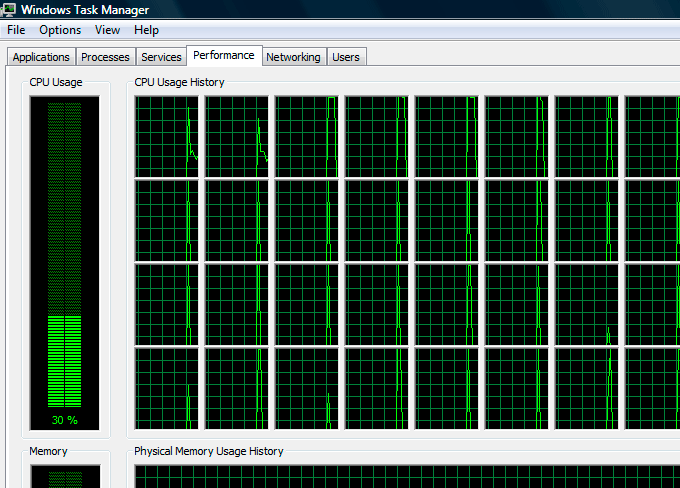
\includegraphics[scale=0.66]{exercises/taskmgr_64cpu_crop.png}
\caption{\IFRU{Обманутый}{Fooled} Windows Task Manager}
\end{figure}
% to be proofreaded (end)

\section{\IFRU{Средний уровень}{Middle level}}

\subsection{\Exercise 2.1}

\IFRU{Довольно известный алгоритм, также включен в стандартную библиотеку Си. Исходник взят из glibc 2.11.1. 
Скомпилирован в GCC 4.4.1 с ключом \TT{-Os} (оптимизация по размеру кода). 
Листинг сделан дизассемблером IDA 4.9 из ELF-файла созданным GCC и линкером.}
{Well-known algorithm, also included in standard C library. Source code was taken from glibc 2.11.1.
Compiled in GCC 4.4.1 with \TT{-Os} option (code size optimization).
Listing was done by IDA 4.9 disassembler from ELF-file generated by GCC and linker.}

\IFRU{Для тех кто хочет использовать IDA в процессе изучения, вот здесь лежат .elf и .idb файлы, 
.idb можно открыть при помощи бесплатной IDA 4.9:}
{For those who wants use IDA while learning, here you may find .elf and .idb files,
.idb can be opened with freeware IDA 4.9:}

\url{http://yurichev.com/RE-exercises/middle/1/}

\lstinputlisting{exercises/2_1_gcc.asm}

\subsection{\Exercise 2.2}

\IFRU{Имеется небольшой исполняемый файл, внутри которого находится довольно известная криптосистема}
{There is a small executable file with a well-known cryptosystem inside}.
\IFRU{Попробуйте её идентифицировать}{Try to identify it}.

\begin{itemize}
\item
\href{http://yurichev.com/RE-exercises/middle/2/unknown_cryptosystem.exe}{Windows x86}

\item
\href{http://yurichev.com/RE-exercises/middle/2/unknown_encryption_linux86.tar}{Linux x86}

\item
\href{http://yurichev.com/RE-exercises/middle/2/unknown_encryption_MacOSX.tar}{MacOSX (x64)}
\end{itemize}

\subsection{\Exercise 2.3}

\IFRU{Имеется небольшой исполняемый файл, некая утилита}
{There is a small executable file, some utility}.
\IFRU{Она открывает другой файл, читает его, что-то вычисляет и показывает число с плавающей точкой}
{It opens another file, reads it, calculate something and prints a float number}.
\IFRU{Попробуйте разобраться, что она делает}{Try to understand what it do}.

\begin{itemize}
\item
\href{http://yurichev.com/RE-exercises/middle/3/unknown_utility_2_3.exe}{Windows x86}

\item
\href{http://yurichev.com/RE-exercises/middle/3/unknown_utility_2_3_Linux86.tar}{Linux x86}

\item
\href{http://yurichev.com/RE-exercises/middle/3/unknown_utility_2_3_MacOSX.tar}{MacOSX (x64)}
\end{itemize}

\subsection{\Exercise 2.4}

\IFRU{Утилита, шифрующая и дешифрующая файлы, по паролю}
{There is an utility which encrypts/decrypts files, by password}.
\IFRU{Есть зашифрованный текстовый файл, пароль неизвестен}{There is an encrypted text file,
password is unknown}.
\IFRU{Зашифрованный файл ~--- это текст на английском языке}{Encrypted file is a text in English language}.
\IFRU{Утилита использует сравнительно мощный алгоритм шифрования, тем не менее,
он был применен с очень грубой ошибкой. И из-за ошибки расшифровать файл вполне возможно с минимумом затрат}
{The utility uses relatively strong cryptosystem, nevertheless, it was implemented with a serious blunder.
Since the mistake present, it is possible to decrypt the file with a little effort.}.

\IFRU{Попробуйте найти ошибку и расшифровать файл}{Try to find the mistake and decrypt the file}.

\begin{itemize}
\item
\href{http://yurichev.com/RE-exercises/middle/4/amateur_cryptor.exe}{Windows x86}

\item
\href{http://yurichev.com/RE-exercises/middle/4/text_encrypted}{\IFRU{Текстовый файл}{Text file}}
\end{itemize}

\subsection{\Exercise 2.5}

\IFRU{Это имитация защиты от копирования использующей ключевой файл}
{This is software copy protection imitation, which uses key file}.
\IFRU{В ключевом файле имя пользователя и серийный номер}
{The key file contain user (or customer) name and serial number}.

\IFRU{Задачи две}{There are two tasks}:

\begin{itemize}
\item
\IFRU{(Простая) при помощи \tracer либо иного отладчика, 
заставьте эту программу принимать измененный ключевой файл}{(Easy) with the help of \tracer
or any other debugger, force the program to accept changed key file}.

\item
\IFRU{(Средняя) ваша задача заключается в том, чтобы изменить в файле имя пользователя на другое, 
но при этом, модифицировать саму программу нельзя}
{(Medium) your goal is to modify user name to another, however, it is not allowed to patch the program}.
\end{itemize}

\begin{itemize}
\item
\href{http://yurichev.com/RE-exercises/middle/5/super_mega_protection.exe}{Windows x86}

\item
\href{http://yurichev.com/RE-exercises/middle/5/super_mega_protection.tar}{Linux x86}

\item
\href{http://yurichev.com/RE-exercises/middle/5/super_mega_protection_MacOSX.tar}{MacOSX (x64)}

\item
\href{http://yurichev.com/RE-exercises/middle/5/sample.key}{\IFRU{Ключевой файл}{Key file}}
\end{itemize}

\subsection{\Exercise 2.6}

\IFRU{Это очень примитивный игрушечный веб-сервер, поддерживающий только статические файлы, без \ac{CGI}, и т.д}
{Here is a very primitive toy web-server, supporting only static files, without \ac{CGI}, etc}.
\IFRU{В нем сознательно оставлено по крайней мере 4 уязвимости}
{At least 4 vulnerabilities are leaved here intentionally}.
\IFRU{Постарайтесь найти их все и использовать для взлома удаленной машины}
{Try to find them all and exploit them in order for breaking into a remote host}.

\begin{itemize}
\item
\href{http://yurichev.com/RE-exercises/middle/6/webserv_win32.rar}{Windows x86}

\item
\href{http://yurichev.com/RE-exercises/middle/6/webserv_Linux_x86.tar}{Linux x86}

\item
\href{http://yurichev.com/RE-exercises/middle/6/webserv_MacOSX_x64.tar}{MacOSX (x64)}
\end{itemize}

\subsection{\Exercise 2.7}

% to be proofreaded (begin)
\IFRU{При помощи \tracer или любого другого win32-отладчика, найдите скрытые мины во время игры,
в стандартной игре Windows MineSweeper}
{With the help of \tracer or any other win32 debugger, reveal hidden mines in the MineSweeper standard Widnows game
during play}.

\IFRU{Подсказка: в}{Hint:} \cite{trew} \IFRU{имеются некоторые описания внутренностей игры MineSweeper}
{have some insights about MineSweeper's internals}.
% to be proofreaded (end)

\section{crackme / keygenme}

\IFRU{Несколько моих \gls{keygenme}:}
{Couple of my \glspl{keygenme}:}

\url{http://crackmes.de/users/yonkie/}

